\section{Appendix}

\subsubsection{Appendix 1 (Data Collection)}

\begin{center}
    \centering
    \begin{figure}[H]
        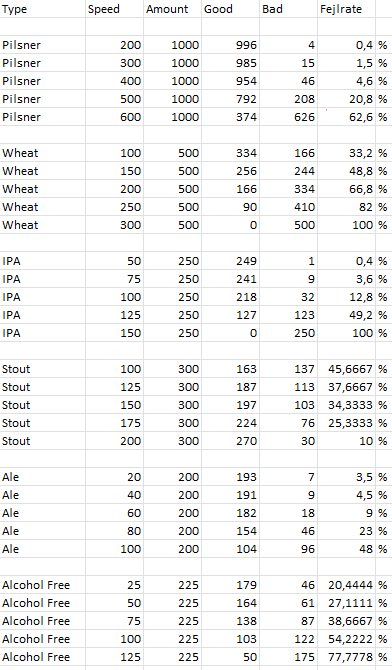
\includegraphics[width=0.6\textwidth]{img/datacollection.png}
        \caption{All the data gathered from the tests}
        \label{fig:datacollection}
    \end{figure}
  \end{center}

\newpage
\subsubsection{Appendix 2 (OPC-client.js)}

\begin{center}
    \begin{minted}[linenos, breaklines, firstnumber=last]{javascript}
        const { OPCUAClient, DataType, AttributeIds, WriteValueOptions, ClientSubscription } = require('node-opcua-client')
        const { MonitoringMode } = require('node-opcua-types')
        const { TimestampsToReturn } = require('node-opcua-data-value')
        let session // OPC session
        let client // OPC client
        let stateSubscription // OPC subscription
        let stopReasonSubscription // OPC subscription
        let batchId = 0
        let batchIdFromOPC = 0
        let currentState

        const PackMLCmdOptions = {
            Reset: 1,
            Start: 2,
            Stop: 3,
            Abort: 4,
            Clear: 5,
        }

        const PackMLStateOptions = {
            Deactivated: 0,
            Clearing: 1,
            Stopped: 2,
            Starting: 3,
            Idle: 4,
            Suspended: 5,
            Execute: 6,
            Stopping: 7,
            Aborting: 8,
            Aborted: 9,
            Holding: 10,
            Held: 11,
            Resetting: 15,
            Completing: 16,
            Complete: 17,
            Deactivating: 18,
            Activating: 19,
        }
        module.exports.PackMLStateOptions = PackMLStateOptions

        const variables = [
            { name: 'Temperature', path: 'ns=6;s=::Program:Data.Value.Temperature' },
            {
                name: 'StateCurrent',
                path: 'ns=6;s=::Program:Cube.Status.StateCurrent',
            },
            { name: 'Vibration', path: 'ns=6;s=::Program:Data.Value.Vibration' },
            { name: 'Barley', path: 'ns=6;s=::Program:Inventory.Barley' },
            { name: 'Hops', path: 'ns=6;s=::Program:Inventory.Hops' },
            { name: 'Malt', path: 'ns=6;s=::Program:Inventory.Malt' },
            { name: 'Wheat', path: 'ns=6;s=::Program:Inventory.Wheat' },
            { name: 'Yeast', path: 'ns=6;s=::Program:Inventory.Yeast' },
            { name: 'FillingInventory', path: 'ns=6;s=::Program:FillingInventory' },
            { name: 'Counter', path: 'ns=6;s=::Program:Maintenance.Counter' },
            { name: 'State', path: 'ns=6;s=::Program:Maintenance.State' },
            { name: 'ExecuteState', path: 'ns=6;s=::Program:Cube.Command.CmdChangeRequest' },
            { name: 'ExecuteOrder', path: 'ns=6;s=::Program:Cube.Command.CntrlCmd' },
            { name: 'StopReason', path: 'ns=6;s=::Program:Cube.Admin.StopReason.ID' },
            { name: 'BeerType', path: 'ns=6;s=::Program:Cube.Command.Parameter[1].Value' },
            { name: 'BeerAmount', path: 'ns=6;s=::Program:Cube.Command.Parameter[2].Value' },
            { name: 'MachineSpeed', path: 'ns=6;s=::Program:Cube.Command.MachSpeed' },
            { name: 'SetBatchId', path: 'ns=6;s=::Program:Cube.Command.Parameter[0].Value' },
            { name: 'BatchId', path: 'ns=6;s=::Program:Cube.Status.Parameter[0].Value' },
        ]

        const products = {
            Pilsner: 0,
            Wheat: 1,
            IPA: 2,
            Stout: 3,
            Ale: 4,
            'Alcohol Free': 5,
        }

        const speedLimits = {
            [products.Pilsner]: 263,
            [products.Wheat]: 5,
            [products.IPA]: 58,
            [products.Stout]: 200,
            [products.Ale]: 1,
            [products['Alcohol Free']]: 1,
        }

        function findVariable(name) {
            return variables.find((v) => v.name === name)
        }

        const opcEndpointUrl = process.env.OPC_URL || 'opc.tcp://127.0.0.1:4840'

        module.exports = {
            getBatchId: () => batchIdFromOPC,
            getStateCurrent: () => currentState,
            connect: async () => {
                try {
                    if (session) {
                        console.log('Session already created!')
                        return
                    }
                    client = OPCUAClient.create({
                        endpointMustExist: false,
                    })
                    console.log('Connecting to OPC UA server... !!!', opcEndpointUrl)
                    await client.connect(opcEndpointUrl).then(() => console.log('Session created!'))
                    session = await client.createSession()
                    // make subcribe if there is none
                    if (!stateSubscription) {
                        module.exports.subscribe('StateCurrent', (value) => {
                            const currentValue = value.value
                            if (currentValue !== currentState) {
                                console.log('State changed to', currentValue)
                                currentState = currentValue
                            }
                        })
                    }

                    if (!stopReasonSubscription) {
                        module.exports.subscribe('StopReason', (value) => {
                            const currentValue = value.value
                            if (currentValue !== currentState) {
                                currentState = currentValue
                                this.maintenence()
                            }
                        })
                    }
                } catch (err) {
                    if (err instanceof Error) {
                        console.log(err.message)
                    }
                }
            },

            /**
             * @param {"Temperature"|"StateCurrent"|"Vibration"|"Barley"|"Hops"|"Malt"|"Wheat"|"Yeast"|"FillingInventory"|"Counter"|"State"|"StopReason"|"ExecuteState"|"ExecuteOrder"|"BeerType"|"BeerAmount"|"MachineSpeed"|"BatchId"|"SetBatchId"} VariableName - "Temperature
             * @returns {Promise<Number> | undefined}
             */
            read: async (VariableName) => {
                const variable = findVariable(VariableName)
                if (variable) {
                    const value = await session.readVariableValue(variable.path)
                    //console.log(`Read from node ${VariableName} with value ${value.value.value}`)
                    return value.value.value
                } else {
                    console.error(`Variable ${VariableName} not found`)
                }
            },

            /**
             * @param {"Temperature"|"StateCurrent"|"Vibration"|"Barley"|"Hops"|"Malt"|"Wheat"|"Yeast"|"FillingInventory"|"Counter"|"State"|"StopReason"|"ExecuteState"|"ExecuteOrder"|"BeerType"|"BeerAmount"|"MachineSpeed"|"BatchId"|"SetBatchId"} VariableName - "Temperature
             * @param value
             * @param {number} dataType
             */
            write: async (VariableName, value, dataType) => {
                if (Object.values(DataType).indexOf(dataType) === -1) {
                    throw new Error('Invalid data type')
                }

                const variable = findVariable(VariableName)

                if (!variable) {
                    throw new Error(`Variable ${VariableName} not found`)
                }
                const nodeToWrite = {
                    nodeId: variable.path,
                    attributeId: AttributeIds.Value,
                    value: {
                        value: {
                            dataType: dataType,
                            value: value,
                        },
                    },
                }

                const statusCode = await session.write(nodeToWrite)
                console.log(`Writing to node ${VariableName} with value ${value}`)
                if (statusCode._value !== 0) throw new Error(`Write failed with status code ${statusCode.toString()}`)
                console.log(`Written to node ${VariableName} with status code ${statusCode.toString()}`)
                return statusCode
            },

            maintenence: async () => {
                const StopReason = await module.exports.read('StopReason')
                let Products = []
                if (StopReason === 11) {
                    await module.exports.write('ExecuteOrder', 1, DataType.Int16)
                    await module.exports.write('ExecuteState', true, DataType.Boolean)
                    await module.exports.write('ExecuteOrder', 2, DataType.Int16)
                    await module.exports.write('ExecuteState', true, DataType.Boolean)
                    await module.exports.write('ExecuteOrder', 3, DataType.Int16)
                    await module.exports.write('ExecuteState', true, DataType.Boolean)
                    await module.exports.write('ExecuteOrder', 4, DataType.Int16)
                    await module.exports.write('ExecuteState', true, DataType.Boolean)
                    return true
                } else if (StopReason === 10) {
                    await module.exports.write('FillingInventory', true, DataType.Boolean)
                    while ((await module.exports.read('FillingInventory')) === true) {
                        Products = await Promise.all([
                            module.exports.read('Yeast'),
                            module.exports.read('Barley'),
                            module.exports.read('Wheat'),
                            module.exports.read('Malt'),
                            module.exports.read('Hops'),
                        ])
                        let Isfull = true
                        Products.forEach((element) => {
                            if (element < 30000) {
                                Isfull = false
                            }
                        })
                        if (Isfull === true) {
                            await module.exports.write('FillingInventory', false, DataType.Boolean)
                        }
                    }
                    return true
                }
                console.log('No maintenence needed')
                return false
            },

            /**
             *
             * @param {0|1|2|3|4|5} beer_type
             * @param {number} beer_amount
             * @param {number} machine_speed
             * @returns {Promise<boolean>}
             */
            brew: async (beer_type, beer_amount, machine_speed) => {
                try {
                    if (beer_type === undefined || !beer_amount || !machine_speed) {
                        console.error('Missing required fields')
                        return false
                    }

                    if (Object.values(products).indexOf(beer_type) === -1) {
                        console.error('Invalid beer type')
                        return false
                    }

                    /*
                    const maxMachineSpeedForBeerType = speedLimits[beer_type]

                    if (machine_speed < 0 || machine_speed > maxMachineSpeedForBeerType) {
                        console.error(`Invalid machine speed for ${beer_type}. It should be between 0 and ${speedLimits[beer_type]}.`)
                        return false
                    }
                    */
                    machine_speed = speedLimits[beer_type];

                    const nodesToWrite = [
                        {
                            variable: 'BeerType',
                            dataType: DataType.Float,
                            value: beer_type,
                        },
                        {
                            variable: 'BeerAmount',
                            dataType: DataType.Float,
                            value: beer_amount,
                        },
                        {
                            variable: 'MachineSpeed',
                            dataType: DataType.Float,
                            value: machine_speed,
                        },
                    ]

                    let state = await module.exports.read('StateCurrent')
                    if (state !== PackMLStateOptions.Execute) {
                        console.log('PackMLStateHandler Brew')
                        await PackMLStateHandler()
                    }

                    const currentStopReason = await module.exports.read('StopReason')
                    const needsMaintenance = currentStopReason === 10 || currentStopReason === 11

                    if (needsMaintenance) await module.exports.maintenence()

                    for (let node of nodesToWrite) {
                        const StopReason = await module.exports.read('StopReason')
                        if (StopReason === 10 || StopReason === 11) {
                            await module.exports.maintenence()
                        }
                        await module.exports.write(node.variable, node.value, node.dataType)
                    }

                    batchId++
                    console.log('Value changed for batchId to ', batchId)
                    await module.exports.write('SetBatchId', batchId, DataType.Float)

                    console.log(`Brewing ${beer_amount} of beer type ${beer_type} at a speed of ${machine_speed} beers per minute`)
                    state = await module.exports.read('StateCurrent')
                    if (state !== PackMLStateOptions.Execute) {
                        console.log('PackMLStateHandler Brew')
                        await PackMLStateHandler()
                    }
                    return true
                } catch (err) {
                    console.error('An error occurred while brewing:', err)
                    return false
                }
            },

            disconnect: async () => {
                try {
                    await session.close()
                    await client.disconnect()
                    session = null
                    client = null
                    console.log('Session closed!')
                } catch (err) {
                    if (err instanceof Error) {
                        console.log(err.message)
                    }
                    process.exit(0)
                }
            },
            subscribe: (VariableName, callback) => {
                const variable = findVariable(VariableName)
                if (!variable) {
                    throw new Error(`Variable ${VariableName} not found`)
                }

                if (!session) {
                    throw new Error('Session not created')
                }

                console.log('Subscribing to node', variable.path)

                stateSubscription = ClientSubscription.create(session, {
                    requestedPublishingInterval: 1000,
                    requestedMaxKeepAliveCount: 20,
                    requestedLifetimeCount: 6000,
                    maxNotificationsPerPublish: 1000,
                    publishingEnabled: true,
                    priority: 10,
                })

                stateSubscription.monitor(
                    {
                        nodeId: variable.path,
                        attributeId: AttributeIds.Value,
                    },
                    {
                        samplingInterval: 100,
                        discardOldest: true,
                        queueSize: 10,
                    },
                    TimestampsToReturn.Both,
                    MonitoringMode.Reporting
                )

                stateSubscription.on('received_notifications', (notifications) => {
                    console.log(
                        'Received notifications',
                        variable.name,
                        variable.path,
                        notifications.notificationData[0].monitoredItems[0].value.value
                    )
                    callback(notifications.notificationData[0].monitoredItems[0].value.value)
                })
            },
        }

        async function PackMLStateHandler() {
            console.log('PackMLStateHandler')
            const state = await module.exports.read('StateCurrent')
            switch (state) {
                case PackMLStateOptions.Deactivated: {
                    break
                }
                case PackMLStateOptions.Clearing: {
                    break
                }
                case PackMLStateOptions.Stopped: {
                    await module.exports.write('ExecuteOrder', PackMLCmdOptions.Reset, DataType.Int16)
                    await module.exports.write('ExecuteState', true, DataType.Boolean)
                    await new Promise((resolve) => setTimeout(resolve, 1000))
                    await module.exports.write('ExecuteOrder', PackMLCmdOptions.Start, DataType.Int16)
                    await module.exports.write('ExecuteState', true, DataType.Boolean)
                    await new Promise((resolve) => setTimeout(resolve, 3000))
                    await module.exports.write('ExecuteOrder', PackMLCmdOptions.Reset, DataType.Int16)
                    await module.exports.write('ExecuteState', true, DataType.Boolean)
                    await new Promise((resolve) => setTimeout(resolve, 1000))
                    break
                }
                case PackMLStateOptions.Starting: {
                    break
                }
                case PackMLStateOptions.Idle: {
                    await new Promise((resolve) => setTimeout(resolve, 1000))
                    await module.exports.write('ExecuteOrder', PackMLCmdOptions.Start, DataType.Int16)
                    await module.exports.write('ExecuteState', true, DataType.Boolean)
                    await new Promise((resolve) => setTimeout(resolve, 3000))
                    await module.exports.write('ExecuteOrder', PackMLCmdOptions.Reset, DataType.Int16)
                    await module.exports.write('ExecuteState', true, DataType.Boolean)
                    await new Promise((resolve) => setTimeout(resolve, 1000))
                    break
                }
                case PackMLStateOptions.Suspended: {
                    break
                }
                case PackMLStateOptions.Execute: {
                    break
                }
                case PackMLStateOptions.Stopping: {
                    break
                }
                case PackMLStateOptions.Aborting: {
                    break
                }
                case PackMLStateOptions.Aborted: {
                    break
                }
                case PackMLStateOptions.Holding: {
                    break
                }
                case PackMLStateOptions.Held: {
                    break
                }
                case PackMLStateOptions.Resetting: {
                    break
                }
                case PackMLStateOptions.Completing: {
                    break
                }
                case PackMLStateOptions.Complete: {
                    // reset then clear
                    await module.exports.write('ExecuteOrder', PackMLCmdOptions.Reset, DataType.Int16)
                    await module.exports.write('ExecuteState', true, DataType.Boolean)
                    await new Promise((resolve) => setTimeout(resolve, 1000))
                    await module.exports.write('ExecuteOrder', PackMLCmdOptions.Clear, DataType.Int16)
                    await module.exports.write('ExecuteState', true, DataType.Boolean)
                    await new Promise((resolve) => setTimeout(resolve, 1000))
                    break
                }
                case PackMLStateOptions.Deactivating: {
                    break
                }
                case PackMLStateOptions.Activating: {
                    break
                }
                default: {
                    throw new Error('Invalid state')
                }
            }
        }

    \end{minted}
\end{center}

\newpage
\subsubsection{Appendix 3 (Index.js)}
\begin{center}
    \begin{minted}[linenos, breaklines, firstnumber=last]{javascript}
        const path = require('path')
        const express = require('express')
        const opcuaClient = require('./OPC/OPC_client')
        const database = require('./db.js')
        const app = express()
        const PORT = process.env.PORT || 3000
        const DIST_DIR = process.env.DIST_DIR || '../frontend/dist'

        app.use(express.static(path.resolve(process.cwd(), DIST_DIR)))
        app.use(express.json())

        app.get('/api/inventory', async (req, res) => {
            res.setHeader('Cache-Control', 'no-cache')
            res.setHeader('Content-Type', 'text/event-stream')
            res.setHeader('Access-Control-Allow-Origin', '*')
            res.setHeader('Connection', 'keep-alive')
            res.flushHeaders() // flush the headers to establish SSE with client

            const opcua = opcuaClient
            await opcua.connect()

            const interval = setInterval(async () => {
                const [wheat, barley, hops, yeast, malt] = await Promise.all([
                    opcua.read('Wheat'),
                    opcua.read('Barley'),
                    opcua.read('Hops'),
                    opcua.read('Yeast'),
                    opcua.read('Malt'),
                ])
                const chunk = JSON.stringify({ wheat, barley, hops, yeast, malt })
                res.write(`data: ${chunk}\n\n`)
            }, 1000)

            res.on('close', () => {
                opcua.disconnect()
                clearInterval(interval)
                res.end()
            })
        })

        app.get('/api/state', async (req, res) => {
            res.setHeader('Cache-Control', 'no-cache')
            res.setHeader('Content-Type', 'text/event-stream')
            res.setHeader('Access-Control-Allow-Origin', '*')
            res.setHeader('Connection', 'keep-alive')
            res.flushHeaders() // flush the headers to establish SSE with client

            const opcua = opcuaClient
            await opcua.connect()

            const interval = setInterval(async () => {
                const state = await opcua.read('State')
                const chunk = JSON.stringify({ state })
                res.write(`data: ${chunk}\n\n`)
            }, 1000)

            res.on('close', () => {
                opcua.disconnect()
                clearInterval(interval)
                res.end()
            })
        })

        const beers = [
            { type: 'Pilsner', id: 0 },
            { type: 'Wheat', id: 1 },
            { type: 'IPA', id: 2 },
            { type: 'Stout', id: 3 },
            { type: 'Ale', id: 4 },
            { type: 'Alcohol Free', id: 5 },
        ]

        app.post('/api/pass-to-queue', async (req, res) => {
            try {
                // check if the request has the required fields
                const { amount, type, speed } = req.body
                if (!amount || !type) throw new Error('Request is missing required fields')

                console.log(`Received request to brew ${amount} of ${type}`)

                // receive request to process a beer type and an amount
                const beer = beers.find((v) => v.type === req.body.type) // search map where beer type equals product
                const beer_type = beer.id // get beer type id

                if (beer_type === undefined) throw new Error('Beer type not found')

                // convert amount to number
                const beer_amount = Number(amount)
                if (isNaN(beer_amount)) throw new Error('Amount is not a number')

                console.log(`Received request to brew ${beer_amount} of ${type}`)

                await opcuaClient.connect()

                const state = opcuaClient.getStateCurrent()
                if (state == 6) throw new Error('Brewing is not possible at the moment')

                if (await opcuaClient.brew(beer_type, beer_amount, speed ?? 10)) {
                    // send beer type request to queue
                    database.write(beer_type, beer_amount)// send data to db
                    res.status(200) // if ok, return status code OK
                    res.send({ status: 'ok' })
                } else {
                    res.status(418) // refuse to brew
                    res.send({ status: 'error', error: 'Brewing failed' })
                }
            } catch (error) {
                console.error(error)
                res.status(500).send({ error: error.message, status: 'error' })
            }
        })

        app.listen(PORT, function () {
            console.log(`Server listening on port ${PORT}`)
        })

        module.exports = app      
    \end{minted}
\end{center}

\newpage
\subsubsection{Appendix 4 (App.jsx)}
\begin{center}
    \begin{minted}[linenos, breaklines, firstnumber=last]{jsx}
        import { useEffect, useState } from 'react'
        import Button from './components/button'
        import Dropdown from './components/dropdown'

        export default function App() {
            const [data, setData] = useState()

            const buttons = [
                {
                    text: 'Reset',
                },
                {
                    text: 'Start',
                },
                {
                    text: 'Stop',
                },
                {
                    text: 'Abort',
                },
                {
                    text: 'Clear',
                },
            ]

            const dropdownOptions = ['barley', 'hops', 'malt', 'wheat', 'yeast']

            useEffect(() => {
                const sse = new EventSource('/api', { withCredentials: true })
                sse.onmessage = (e) => {
                    try {
                        console.log(e.data)
                        setData(JSON.parse(e.data))
                        // console.log(JSON.parse(e.data))
                    } catch (e) {
                        console.error(e)
                    }
                }
                sse.onerror = () => {
                    // error log here
                    sse.close()
                }
                sse.onopen = () => {
                    console.log('sse opened')
                }
                return () => {
                    sse.close()
                }
            }, [])

            function handleButtonClick(button) {
                fetch(`/api/${button.text.toLowerCase()}`, { method: 'POST' })
                    .then((res) => res.json())
                    .then((data) => console.log(data))
            }

            return (
                <div className={'min-h-screen bg-black'}>
                    <div className='p-4 space-y-4'>
                        <h1 className='text-2xl font-bold text-gray-900 dark:text-gray-100'>OPCUA Server Dashboard</h1>
                        <div className='grid grid-cols-2 gap-4'>
                            <div className='p-4 rounded-lg bg-white shadow dark:bg-gray-800'>
                                <h2 className='text-lg font-semibold text-gray-900 dark:text-gray-100'>Temperature</h2>
                                <p className='text-gray-500 dark:text-gray-400'>{data ? '72.5°F' : 'Loading...'}</p>
                            </div>
                            <div className='p-4 rounded-lg bg-white shadow dark:bg-gray-800'>
                                <h2 className='text-lg font-semibold text-gray-900 dark:text-gray-100'>Vibration</h2>
                                <p className='text-gray-500 dark:text-gray-400'>{data ? '15.2Hz' : 'Loading...'}</p>
                            </div>
                            <div className='p-4 rounded-lg bg-white shadow dark:bg-gray-800'>
                                <h2 className='text-lg font-semibold text-gray-900 dark:text-gray-100'>Maintenance Status</h2>
                                <p className='text-gray-500 dark:text-gray-400'>{data ? 'Good' : 'Loading...'}</p>
                            </div>
                            <div className='p-4 rounded-lg bg-white shadow dark:bg-gray-800'>
                                <h2 className='text-lg font-semibold text-gray-900 dark:text-gray-100'>Batches Completed</h2>
                                <p className='text-gray-500 dark:text-gray-400'>{data ? '1200' : 'Loading...'}</p>
                            </div>
                            <div className='p-4 rounded-lg bg-white shadow dark:bg-gray-800'>
                                <h2 className='text-lg font-semibold text-gray-900 dark:text-gray-100'>Batches Failed</h2>
                                <p className='text-gray-500 dark:text-gray-400'>{data ? '5' : 'Loading...'}</p>
                            </div>
                        </div>
                        <div className='flex space-x-4'>
                            {buttons.map((button, index) => (
                                <Button
                                    key={index}
                                    text={button.text}
                                    onClick={() => handleButtonClick(button)}
                                >
                                    {button.text}
                                </Button>
                            ))}
                            <Dropdown options={dropdownOptions} />
                        </div>
                        <div className={'mt-10'}>
                            <pre className={'text-white'}>{JSON.stringify(data, null, 2)}</pre>
                        </div>
                    </div>
                </div>
            )
        }
    \end{minted}
\end{center}

\newpage
\subsubsection{Appendix 5 (Temp.jsx)}
\begin{center}
    \begin{minted}[linenos, breaklines, firstnumber=last]{jsx}
        import { useEffect, useState } from 'react'
        import BeerButtons from './components/beer-components/button/beer-buttons.jsx'
        import BeerContainers from './components/beer-components/container/beer-containers.jsx'
        import StartStopButtons from './components/start-stop-buttons.jsx'

        export default function Temp() {
            const [isActive, setIsActive] = useState(false)

            return (
                <div className={'container mx-auto mt-10 flex flex-col gap-4'}>
                    <BeerButtons setIsActive={setIsActive}/>

                    <div className='w-full h-1 bg-gray-500 my-4' />

                    <div className='w-full flex items-center justify-center'>
                        <ProgressBar
                            isActive={isActive}
                            setIsActive={setIsActive}
                        />
                    </div>
                    <div className='w-full h-1 bg-gray-500 my-4' />
                    <div className={'flex justify-between'}>
                        <StartStopButtons setIsActive={setIsActive} />
                        <BeerContainers />
                    </div>
                </div>
            )
        }

        function ProgressBar({ isActive, setIsActive }) {
            const [progress, setProgress] = useState(0)

            useEffect(() => {
                if (isActive) {
                    const state = new EventSource('/api/state')
                    let currentState

                    state.onmessage = function (event) {
                        console.log('event', event.data)
                        currentState = JSON.parse(event.data)
                    }

                    if(currentState != 6) {
                        setIsActive(false)
                    }
                    
                }
            }, [isActive, setIsActive])

            useEffect(() => {
                if (isActive) {
                    const interval = setInterval(() => {
                        setProgress((progress) => {
                            if (progress >= 100) {
                                clearInterval(interval)
                                setIsActive(false)
                                return 0
                            }
                            return progress + 1
                        })
                    }, 100)
                    return () => clearInterval(interval)
                }
            }, [isActive, setIsActive])

            return (
                <div className='w-full flex flex-col items-center justify-center gap-4'>
                    <progress
                        className={'w-4/6 fill-green-500'}
                        value={progress}
                        max='100'
                    />
                </div>
            )
        }
    \end{minted}
\end{center}

\newpage
\subsubsection{Appendix 6 (db.js)}
\begin{center}
    \begin{minted}[linenos, breaklines, firstnumber=last]{javascript}
        const { Pool } = require('pg')
        require('dotenv').config()

        const pool = new Pool({
            host: process.env.PG_HOST,
            port: process.env.PG_PORT,
            user: process.env.PG_USER,
            password: process.env.PG_PASSWORD,
            database: process.env.PG_DATABASE,
        })

        let client

        module.exports = {
            write: async (beer_type, amount) => {
                await module.exports.connect()
                await pool.query(`INSERT INTO beers (beer_type, amount, time) VALUES ($1, $2, NOW())`, [beer_type, amount])
                module.exports.disconnect()
            },

            read: async (beer_id) => {
                await module.exports.connect()
                return await pool.query(`SELECT * FROM beers WHERE id=${beer_id}`).then(module.exports.disconnect())
            },

            query: async (query) => {
                await module.exports.connect()
                return await pool.query(query).then(module.exports.disconnect())
            },

            connect: async (options) => {
                try {
                    client = await pool.connect()
                    console.log('Connected to database')
                } catch (err) {
                    console.log(err.message)
                    throw err
                }
            },
            disconnect: async () => {
                try {
                    await client.release()
                    console.log('Disconnected from database')
                } catch (err) {
                    console.log(err.message)
                    throw err
                }
            },
        }
    \end{minted}
\end{center}